\subsection{Client-Server}

A \definition{Client-Server Architecture} is a \textbf{network-based computing structure} where responsibilities and operations get \textbf{distributed between clients and servers}. Client-Server Architecture is widely used for network applications such as email, web, online banking, e-commerce, etc.

\begin{flushleft}
    \textcolor{Green3}{\textbf{\faIcon{check} When to use it}}
\end{flushleft}
The three most common cases are:
\begin{itemize}
    \item When \textbf{multiple users} need to access a \textbf{single resource} (e.g. database).

    \item When there is a preexisting software and we must \textbf{access remotely} (e.g. email server).
    
    \item When it is convenient to organize the system around a \textbf{shared piece of functionality used by multiple components} (e.g. authentication or authorization server).
\end{itemize}

\begin{flushleft}
    \textcolor{Red2}{\textbf{\faIcon{exclamation-triangle} Technical issues}}
\end{flushleft}
With this architecture, it's necessary to \textbf{design} and \textbf{document} proper \textbf{interfaces} for our server. It is also necessary to ensure that the server can \textbf{handle multiple simultaneous requests}.

\subsubsection{Interface design}

An \definition{interface design} is a \textbf{boundary} across which components interact. Proper definition of interfaces is an architectural concern (affects maintainability, usability, testability, performance, integrability). There are two important \textbf{guiding principles} for interface design: \textbf{information hiding} and \textbf{low coupling}. An interface should encapsulate a component implementation so that it can be changed without affecting other components.

\highspace
There are several aspects to interface design that need to be considered:
\begin{itemize}
    \item \definition{Contract principle}: any resource (operation, data) added to an interface implies a \textbf{commitment to maintaining} it.

    \item \definition{Least surprise principle}: interfaces should \textbf{behave} consistently \textbf{with expectations}.

    \item \definition{Small interfaces principle}: interfaces should limit the \textbf{exposed resources to the minimum}.
\end{itemize}
There are also some important elements to define: \textbf{interaction style} (e.g. sockets, RPC, REST); \textbf{representation} and structure of exchanged data (affecting expressiveness, interoperability, performance and transparency); \textbf{error handling}.

\newpage

\subsubsection{Error handling, multiple interfaces and interface evolution}

Sometimes there may be some problems, for example: an operation is called with invalid parameters and consequently the call doesn't return anything. This simple example can provoke some scenarios: the component cannot handle the request in its current state; or hardware/software errors prevent successful execution; or there is a misconfiguration issue (e.g. the server is not correctly connected to the database).

There are three possible \textbf{solutions}: \textbf{raising an exception}; \textbf{return an error code} (common); \textbf{log the problem}. There's no single solution, but we can choose several (e.g. error code and log the problem).

\highspace
A \textbf{server} can offer \definition{multiple interfaces} at the same time. This enables separation of concerns, different levels of access rights and support ot \textbf{interface evolution}.

\highspace
\textbf{Interface evolution} occurs for many reasons (e.g. to support new requirements). Several \textbf{strategies} are needed to support continuity:
\begin{itemize}
    \item \textbf{\underline{Deprecation}}: declare well in advance that an interface version will be retired by a certain date;

    \item \textbf{\underline{Versioning}}: maintain multiple active versions of the interface;

    \item \textbf{\underline{Extension}}: a new version extends the previous one.
\end{itemize}

\newpage

\subsubsection{Handling multiple requests}

The server must be able to receive and process requests from multiple clients. There are two main approaches to this: \emph{forking} and \emph{worker pooling}.

\begin{flushleft}
    \large
    \textcolor{Red2}{\textbf{Forking}}
\end{flushleft}
The \definition{forking} approach is the same as that used by the Apache Web Server: \textbf{one process per request or per client}.

\begin{figure}[!htp]
    \centering
    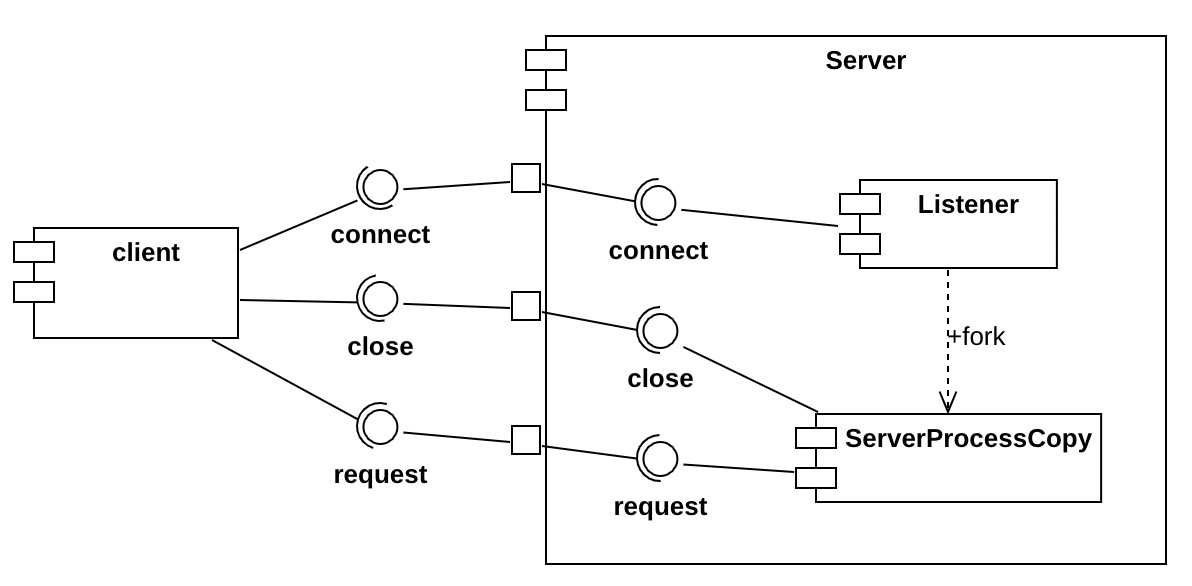
\includegraphics[width=.8\textwidth]{img/forking-1.png}
    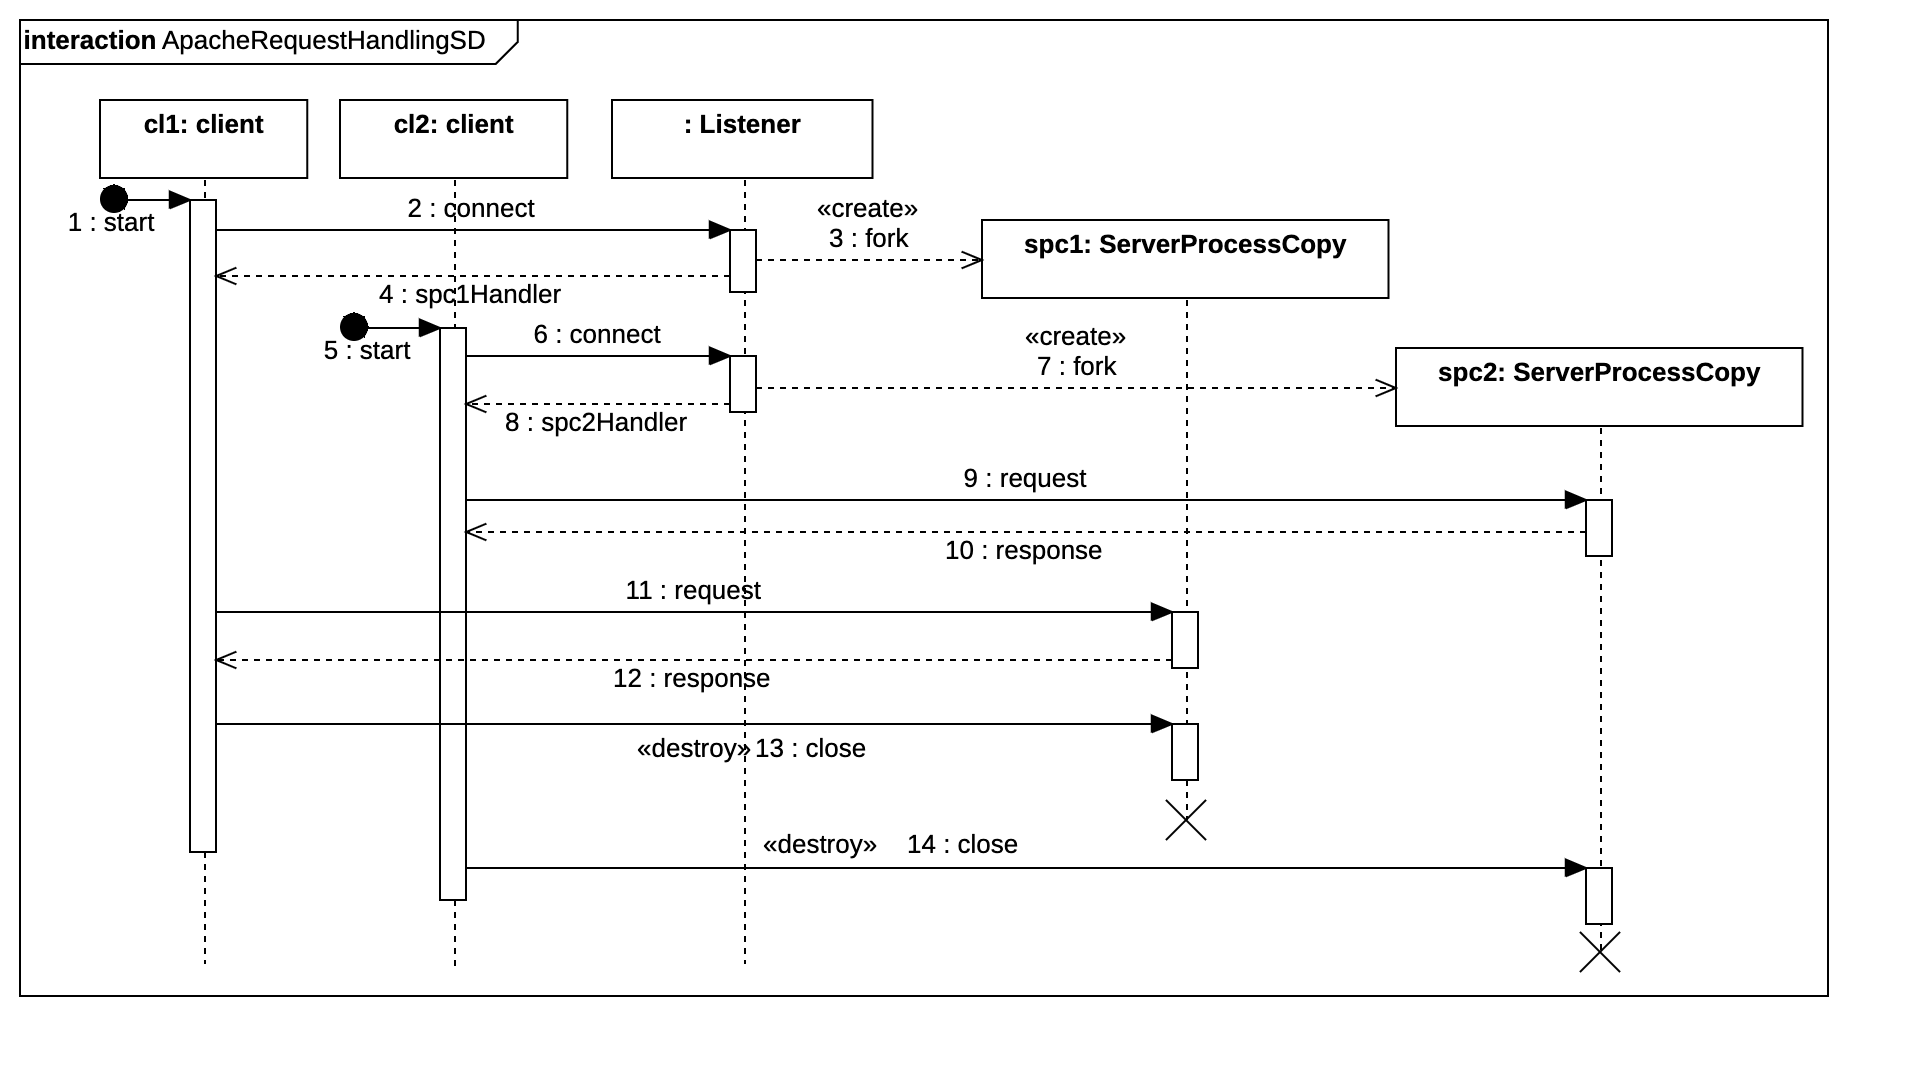
\includegraphics[width=\textwidth]{img/forking-2.png}
    \caption{Forking diagrams.}
\end{figure}

\begin{flushleft}
    \textcolor{Green3}{\textbf{\faIcon{check} Forking Advantages}}
\end{flushleft}
\begin{itemize}
    \item Architectural \textbf{simplicity}.
    
    \item \textbf{Isolation} and \textbf{protection} given by the one-connection-per-process model. Note: slow processes do not affect other incoming connections.
    
    \item \textbf{Simple to program}.
\end{itemize}

\newpage

\begin{flushleft}
    \textcolor{Red2}{\textbf{\faIcon{exclamation-triangle} Forking Issues}}
\end{flushleft}
\begin{itemize}
    \item Growth of the WWW over the last 20 years (number of users and weight of web pages).
    
    \item The number of \textbf{active processes} at time $t$ is \textbf{difficult to predict} and may \textbf{saturate resources}.
    
    \item \textbf{Expensive} fork-kill operations for each \textbf{incoming connection}.
\end{itemize}

\newpage

\begin{flushleft}
    \large
    \textcolor{Red2}{\textbf{Worker pooling}}
\end{flushleft}
It is an alternative approach adopted by NGINX Web Server. It is \textbf{designed for high concurrency} but has to deal with \textbf{scalability issues}.

\begin{figure}[!htp]
    \centering
    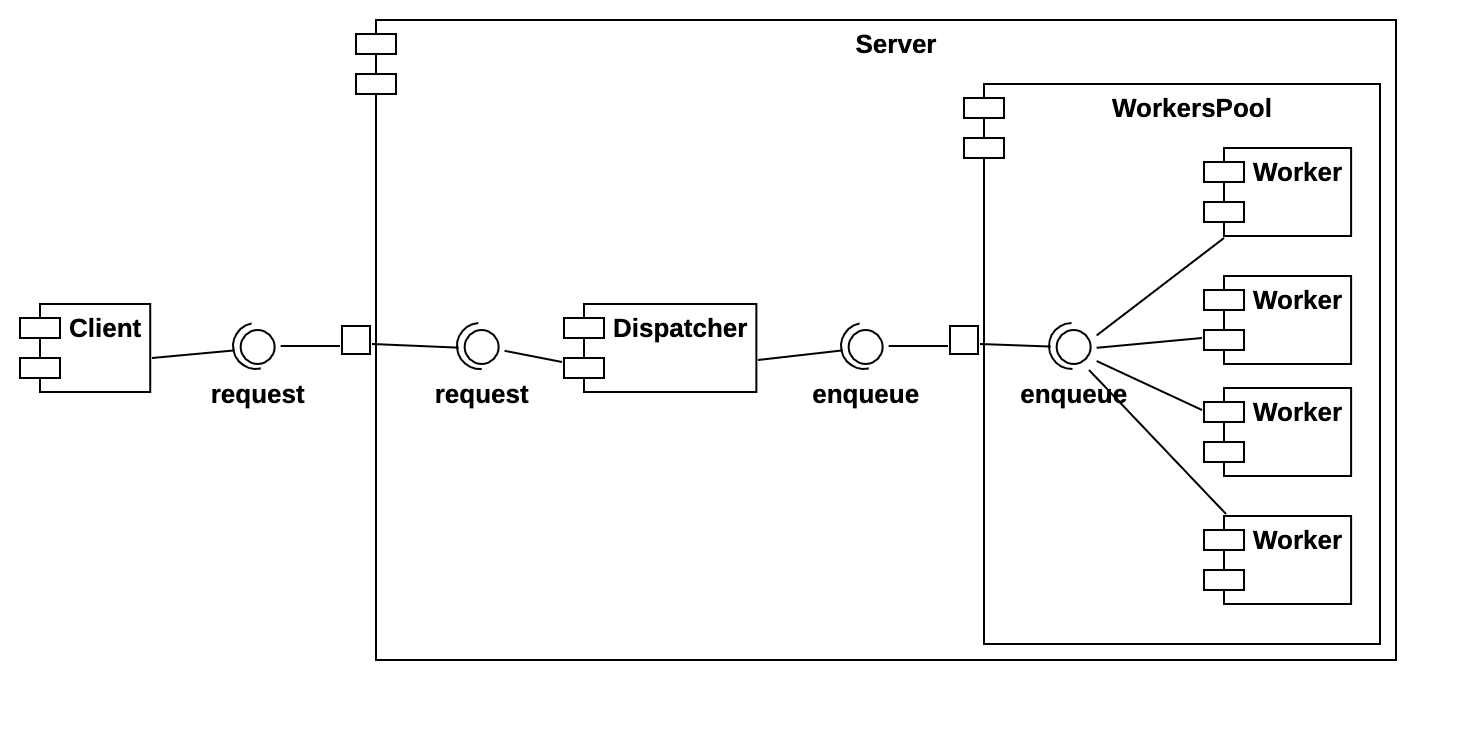
\includegraphics[width=.9\textwidth]{img/worker-pooling-1.png}
    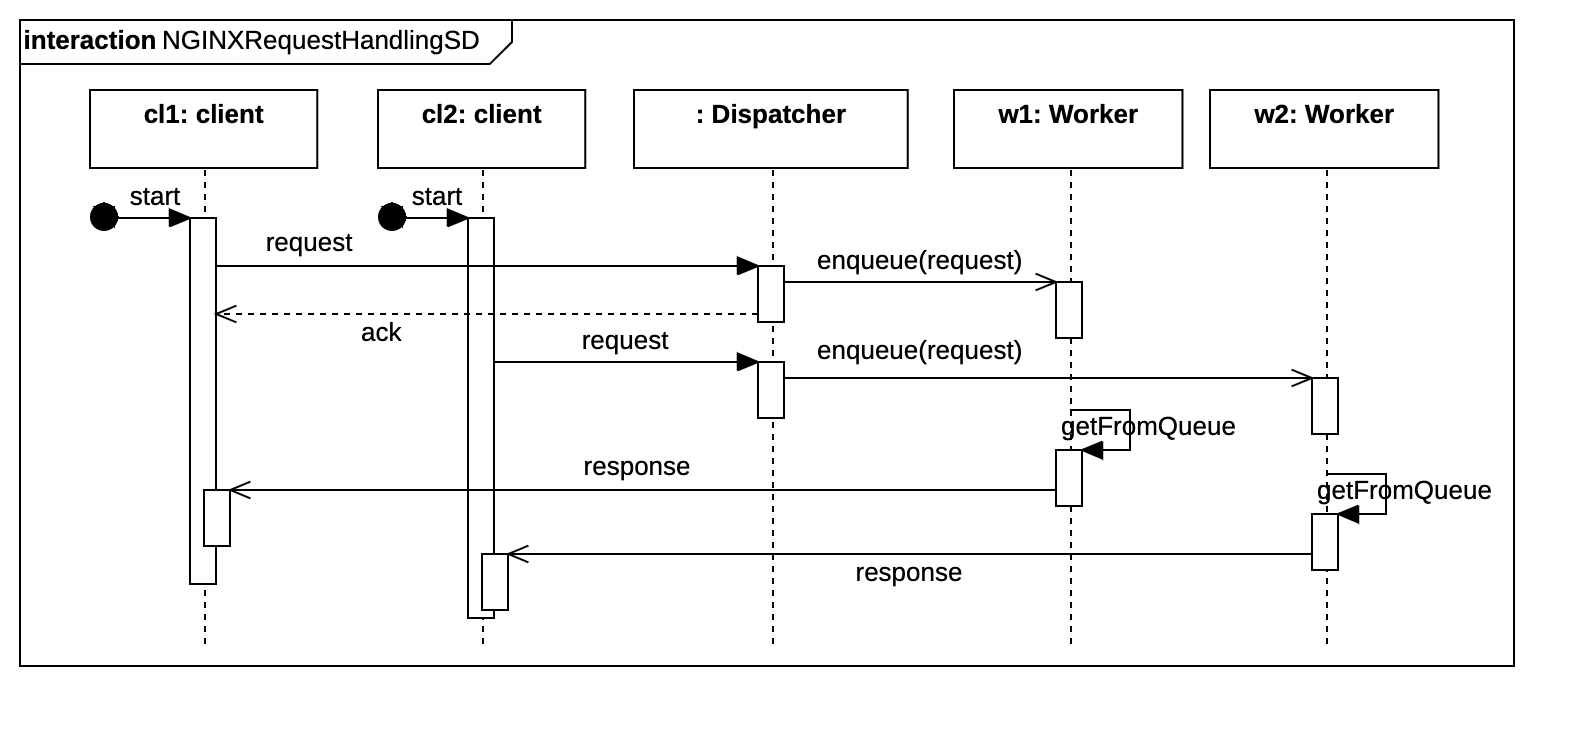
\includegraphics[width=\textwidth]{img/worker-pooling-2.png}
    \caption{Worker pooling diagrams.}
\end{figure}

\noindent
Despite the well-known problem of this architecture (scalability), NGINX addresses the previous problems by introducing a new \textbf{architectural tactic}. A \emph{tactic} is a \textbf{design decision that affects the control of one or more quality attributes}.

\begin{flushleft}
    \textcolor{Green3}{\textbf{\faIcon{check} Worker Pooling Advantages (quality attribute trade-offs)}}
\end{flushleft}
\begin{itemize}
    \item Number of \textbf{workers} is fixed, so they \textbf{do not saturate available resources}.
    
    \item \textbf{Each worker} has a \textbf{queue}.
    
    \item When \textbf{queues} are \textbf{full} the \textbf{dispatcher drops the incoming requests} to keep high performance (\textbf{optimize scalability and performance by sacrificing availability}).
    
    \item Dispatcher \textbf{balances} the \textbf{workload} among available workers \textbf{according to specific policies}.
\end{itemize}